\documentclass[10pt, a4paper, twocolumn]{article}

%%%%%%%%%%%%%%%%%%%%%%%%%%%%%%%%%%%%%%%%%
% Wenneker Article
% Structure Specification File
% Version 1.0 (28/2/17)
%
% This file originates from:
% http://www.LaTeXTemplates.com
%
% Authors:
% Frits Wenneker
% Vel (vel@LaTeXTemplates.com)
%
% License:
% CC BY-NC-SA 3.0 (http://creativecommons.org/licenses/by-nc-sa/3.0/)
%
%%%%%%%%%%%%%%%%%%%%%%%%%%%%%%%%%%%%%%%%%

%----------------------------------------------------------------------------------------
%	PACKAGES AND OTHER DOCUMENT CONFIGURATIONS
%----------------------------------------------------------------------------------------

\usepackage[english]{babel} % English language hyphenation

\usepackage{microtype} % Better typography

\usepackage{amsmath,amsfonts,amsthm} % Math packages for equations

\usepackage[svgnames]{xcolor} % Enabling colors by their 'svgnames'

\usepackage[hang, small, labelfont=bf, up, textfont=it]{caption} % Custom captions under/above tables and figures

\usepackage{booktabs} % Horizontal rules in tables

\usepackage{lastpage} % Used to determine the number of pages in the document (for "Page X of Total")

\usepackage{graphicx} % Required for adding images

\usepackage{enumitem} % Required for customising lists
\setlist{noitemsep} % Remove spacing between bullet/numbered list elements

\usepackage{sectsty} % Enables custom section titles
\allsectionsfont{\usefont{OT1}{phv}{b}{n}} % Change the font of all section commands (Helvetica)

%----------------------------------------------------------------------------------------
%	MARGINS AND SPACING
%----------------------------------------------------------------------------------------

\usepackage{geometry} % Required for adjusting page dimensions

\geometry{
	top=1cm, % Top margin
	bottom=1.5cm, % Bottom margin
	left=2cm, % Left margin
	right=2cm, % Right margin
	includehead, % Include space for a header
	includefoot, % Include space for a footer
	%showframe, % Uncomment to show how the type block is set on the page
}

\setlength{\columnsep}{7mm} % Column separation width

%----------------------------------------------------------------------------------------
%	FONTS
%----------------------------------------------------------------------------------------

\usepackage[T1]{fontenc} % Output font encoding for international characters
\usepackage[utf8]{inputenc} % Required for inputting international characters

\usepackage{XCharter} % Use the XCharter font

%----------------------------------------------------------------------------------------
%	HEADERS AND FOOTERS
%----------------------------------------------------------------------------------------

\usepackage{fancyhdr} % Needed to define custom headers/footers
\pagestyle{fancy} % Enables the custom headers/footers

\renewcommand{\headrulewidth}{0.0pt} % No header rule
\renewcommand{\footrulewidth}{0.4pt} % Thin footer rule

\renewcommand{\sectionmark}[1]{\markboth{#1}{}} % Removes the section number from the header when \leftmark is used

%\nouppercase\leftmark % Add this to one of the lines below if you want a section title in the header/footer

% Headers
\lhead{} % Left header
\chead{\textit{\thetitle}} % Center header - currently printing the article title
\rhead{} % Right header

% Footers
\lfoot{} % Left footer
\cfoot{} % Center footer
\rfoot{\footnotesize Page \thepage\ of \pageref{LastPage}} % Right footer, "Page 1 of 2"

\fancypagestyle{firstpage}{ % Page style for the first page with the title
	\fancyhf{}
	\renewcommand{\footrulewidth}{0pt} % Suppress footer rule
}

%----------------------------------------------------------------------------------------
%	TITLE SECTION
%----------------------------------------------------------------------------------------

\newcommand{\authorstyle}[1]{{\large\usefont{OT1}{phv}{b}{n}\color{DarkRed}#1}} % Authors style (Helvetica)

\newcommand{\institution}[1]{{\footnotesize\usefont{OT1}{phv}{m}{sl}\color{Black}#1}} % Institutions style (Helvetica)

\usepackage{titling} % Allows custom title configuration

\newcommand{\HorRule}{\color{DarkGoldenrod}\rule{\linewidth}{1pt}} % Defines the gold horizontal rule around the title

\pretitle{
	\vspace{-30pt} % Move the entire title section up
	\HorRule\vspace{10pt} % Horizontal rule before the title
	\fontsize{32}{36}\usefont{OT1}{phv}{b}{n}\selectfont % Helvetica
	\color{DarkRed} % Text colour for the title and author(s)
}

\posttitle{\par\vskip 15pt} % Whitespace under the title

\preauthor{} % Anything that will appear before \author is printed

\postauthor{ % Anything that will appear after \author is printed
	\vspace{10pt} % Space before the rule
	\par\HorRule % Horizontal rule after the title
	\vspace{20pt} % Space after the title section
}

%----------------------------------------------------------------------------------------
%	ABSTRACT
%----------------------------------------------------------------------------------------

\usepackage{lettrine} % Package to accentuate the first letter of the text (lettrine)
\usepackage{fix-cm}	% Fixes the height of the lettrine

\newcommand{\initial}[1]{ % Defines the command and style for the lettrine
	\lettrine[lines=3,findent=4pt,nindent=0pt]{% Lettrine takes up 3 lines, the text to the right of it is indented 4pt and further indenting of lines 2+ is stopped
		\color{DarkGoldenrod}% Lettrine colour
		{#1}% The letter
	}{}%
}

\usepackage{xstring} % Required for string manipulation

\newcommand{\lettrineabstract}[1]{
	\StrLeft{#1}{1}[\firstletter] % Capture the first letter of the abstract for the lettrine
	\initial{\firstletter}\textbf{\StrGobbleLeft{#1}{1}} % Print the abstract with the first letter as a lettrine and the rest in bold
}

%----------------------------------------------------------------------------------------
%	BIBLIOGRAPHY
%----------------------------------------------------------------------------------------

\usepackage[backend=bibtex,style=authoryear,natbib=true]{biblatex} % Use the bibtex backend with the authoryear citation style (which resembles APA)

\addbibresource{example.bib} % The filename of the bibliography

\usepackage[autostyle=true]{csquotes} % Required to generate language-dependent quotes in the bibliography

\title{JavaScript}

\author{
	\authorstyle{Boitumelo Phetla\textsuperscript{1,2,3} (PluralSight Google ScholarShip)\textsuperscript{2,3}} % Authors
	\newline\newline % Space before institutions
	\textsuperscript{1}\institution{Universidad Nacional Autónoma de México, Mexico City, Mexico}\\ % Institution 1
	\textsuperscript{2}\institution{University of Texas at Austin, Texas, United States of America}\\ % Institution 2
	\textsuperscript{3}\institution{\texttt{LaTeXTemplates.com}} % Institution 3
}


\date{\today} % Add a date here if you would like one to appear underneath the title block, use \today for the current date, leave empty for no date


\begin{document}
\maketitle % Print the title
\thispagestyle{firstpage} % Apply the page style for the first page (no headers and footers)

%----------------------------------------------------------------------------------------
%	ABSTRACT
%----------------------------------------------------------------------------------------

\lettrineabstract{JavaScript,  is a lightweight interpreted or just-in-time compiled programming language with first-class functions. While it is most well-known as the scripting language for Web pages, many non-browser environments also use it, such as Node.js, Apache CouchDB and Adobe Acrobat.}

%----------------------------------------------------------------------------------------
%	ARTICLE CONTENTS
%----------------------------------------------------------------------------------------

\section{Simplistic JavaScript 1}

\subsection{Command-line based programming}

A simple project: 

\begin{lstlisting}
$bash: touch {index.html,script.js,style.css}
$bash: tree
	__________	index.html
	__________	script.js
	__________	style.css
\end{lstlisting}

Include the script (\textbf{javascript}) and the page styling script (\textbf{cascading stylesheet}) files into the \textit{index.html}.

\begin{lstlisting}
	<head>
			<script src="path/*.js"></script>
			<link rel="stylesheet" href="path/*.css">
	</head>
\end{lstlisting}

Add some simple HTML markup code and launch a live-server of the code. 

\begin{lstlisting}
	<!DOCTYPE>
	<html>
			<head>
					<script src="script.js"></script>
					<link rel="stylesheet" href="style.css">
			</head>
					<body>
							<div id="header">
									<h1>Welcome to JavaScript</h1>
							</div>
					</body>
	</html>
\end{lstlisting}

Launch the command-line (Terminal)

\begin{lstlisting}
$bash: live-server
\end{lstlisting}

\begin{figure}[h!]
	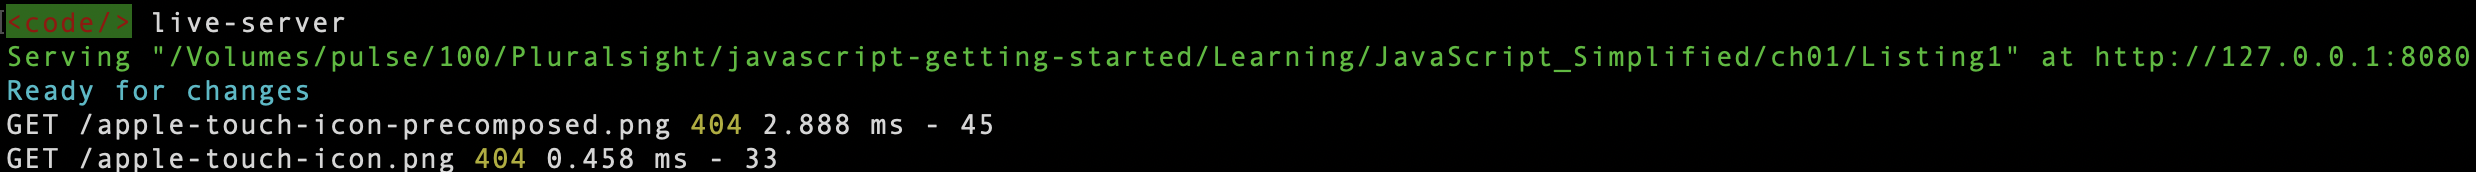
\includegraphics[width=\linewidth]{liveserver.png} % Figure image
	\caption{Live-server} % Figure caption
	\label{ls} % Label for referencing with \ref{bear}
\end{figure}

\subsection{\href{http://plnkr.co}{Plunker}}

Or create an account on  \href{http://plnkr.co/edit/?p=catalogue}{Plunker}.  Plunker sets up your working environment for you.

\begin{figure}[h!]
	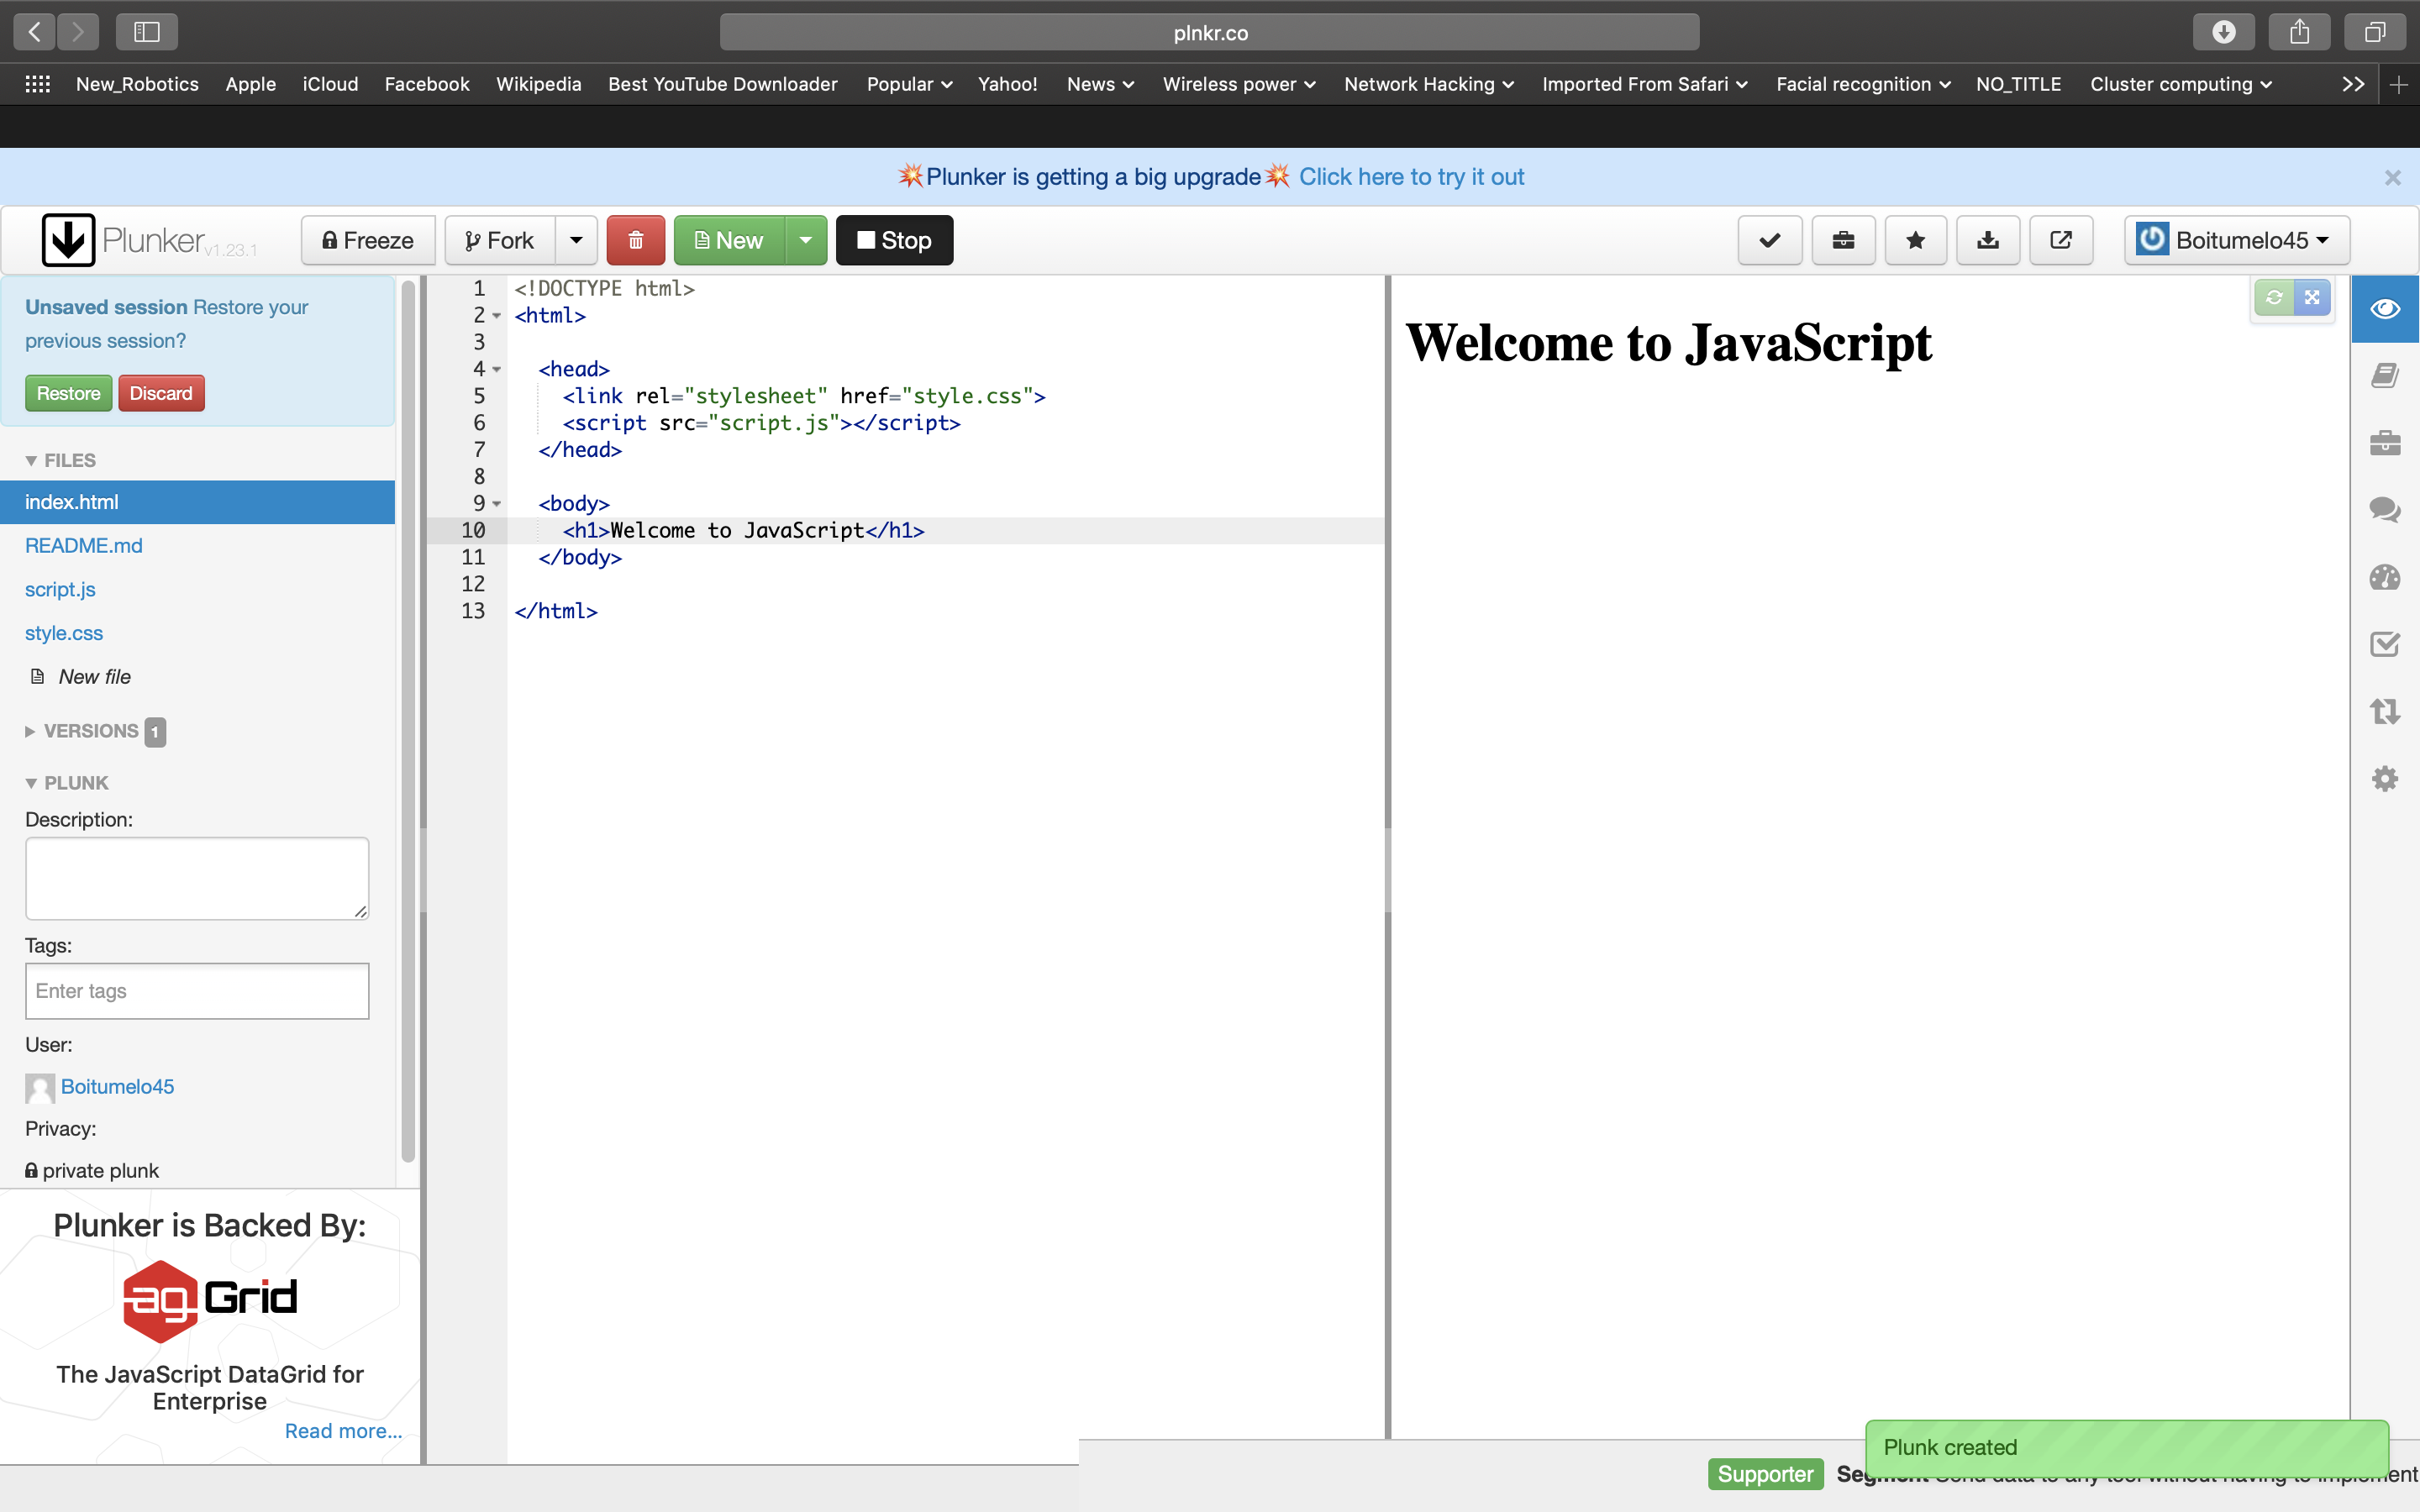
\includegraphics[width=0.89\linewidth]{plunker.png} % Figure image
	\caption{Plunker} % Figure caption
	\label{plnkr} % Label for referencing with \ref{bear}
\end{figure}

\subsection{\href{https://electronjs.org}{Electron}}

Watch this video \href{https://www.youtube.com/watch?v=8YP_nOCO-4Q&feature=youtu.be}{Electron}.

\begin{lstlisting}
# Clone the Quick Start repository
$ git clone https://github.com/electron/electron-quick-start

# Go into the repository
$ cd electron-quick-start

# Install the dependencies and run
$ npm install && npm start
\end{lstlisting}

\begin{figure}[h!]
	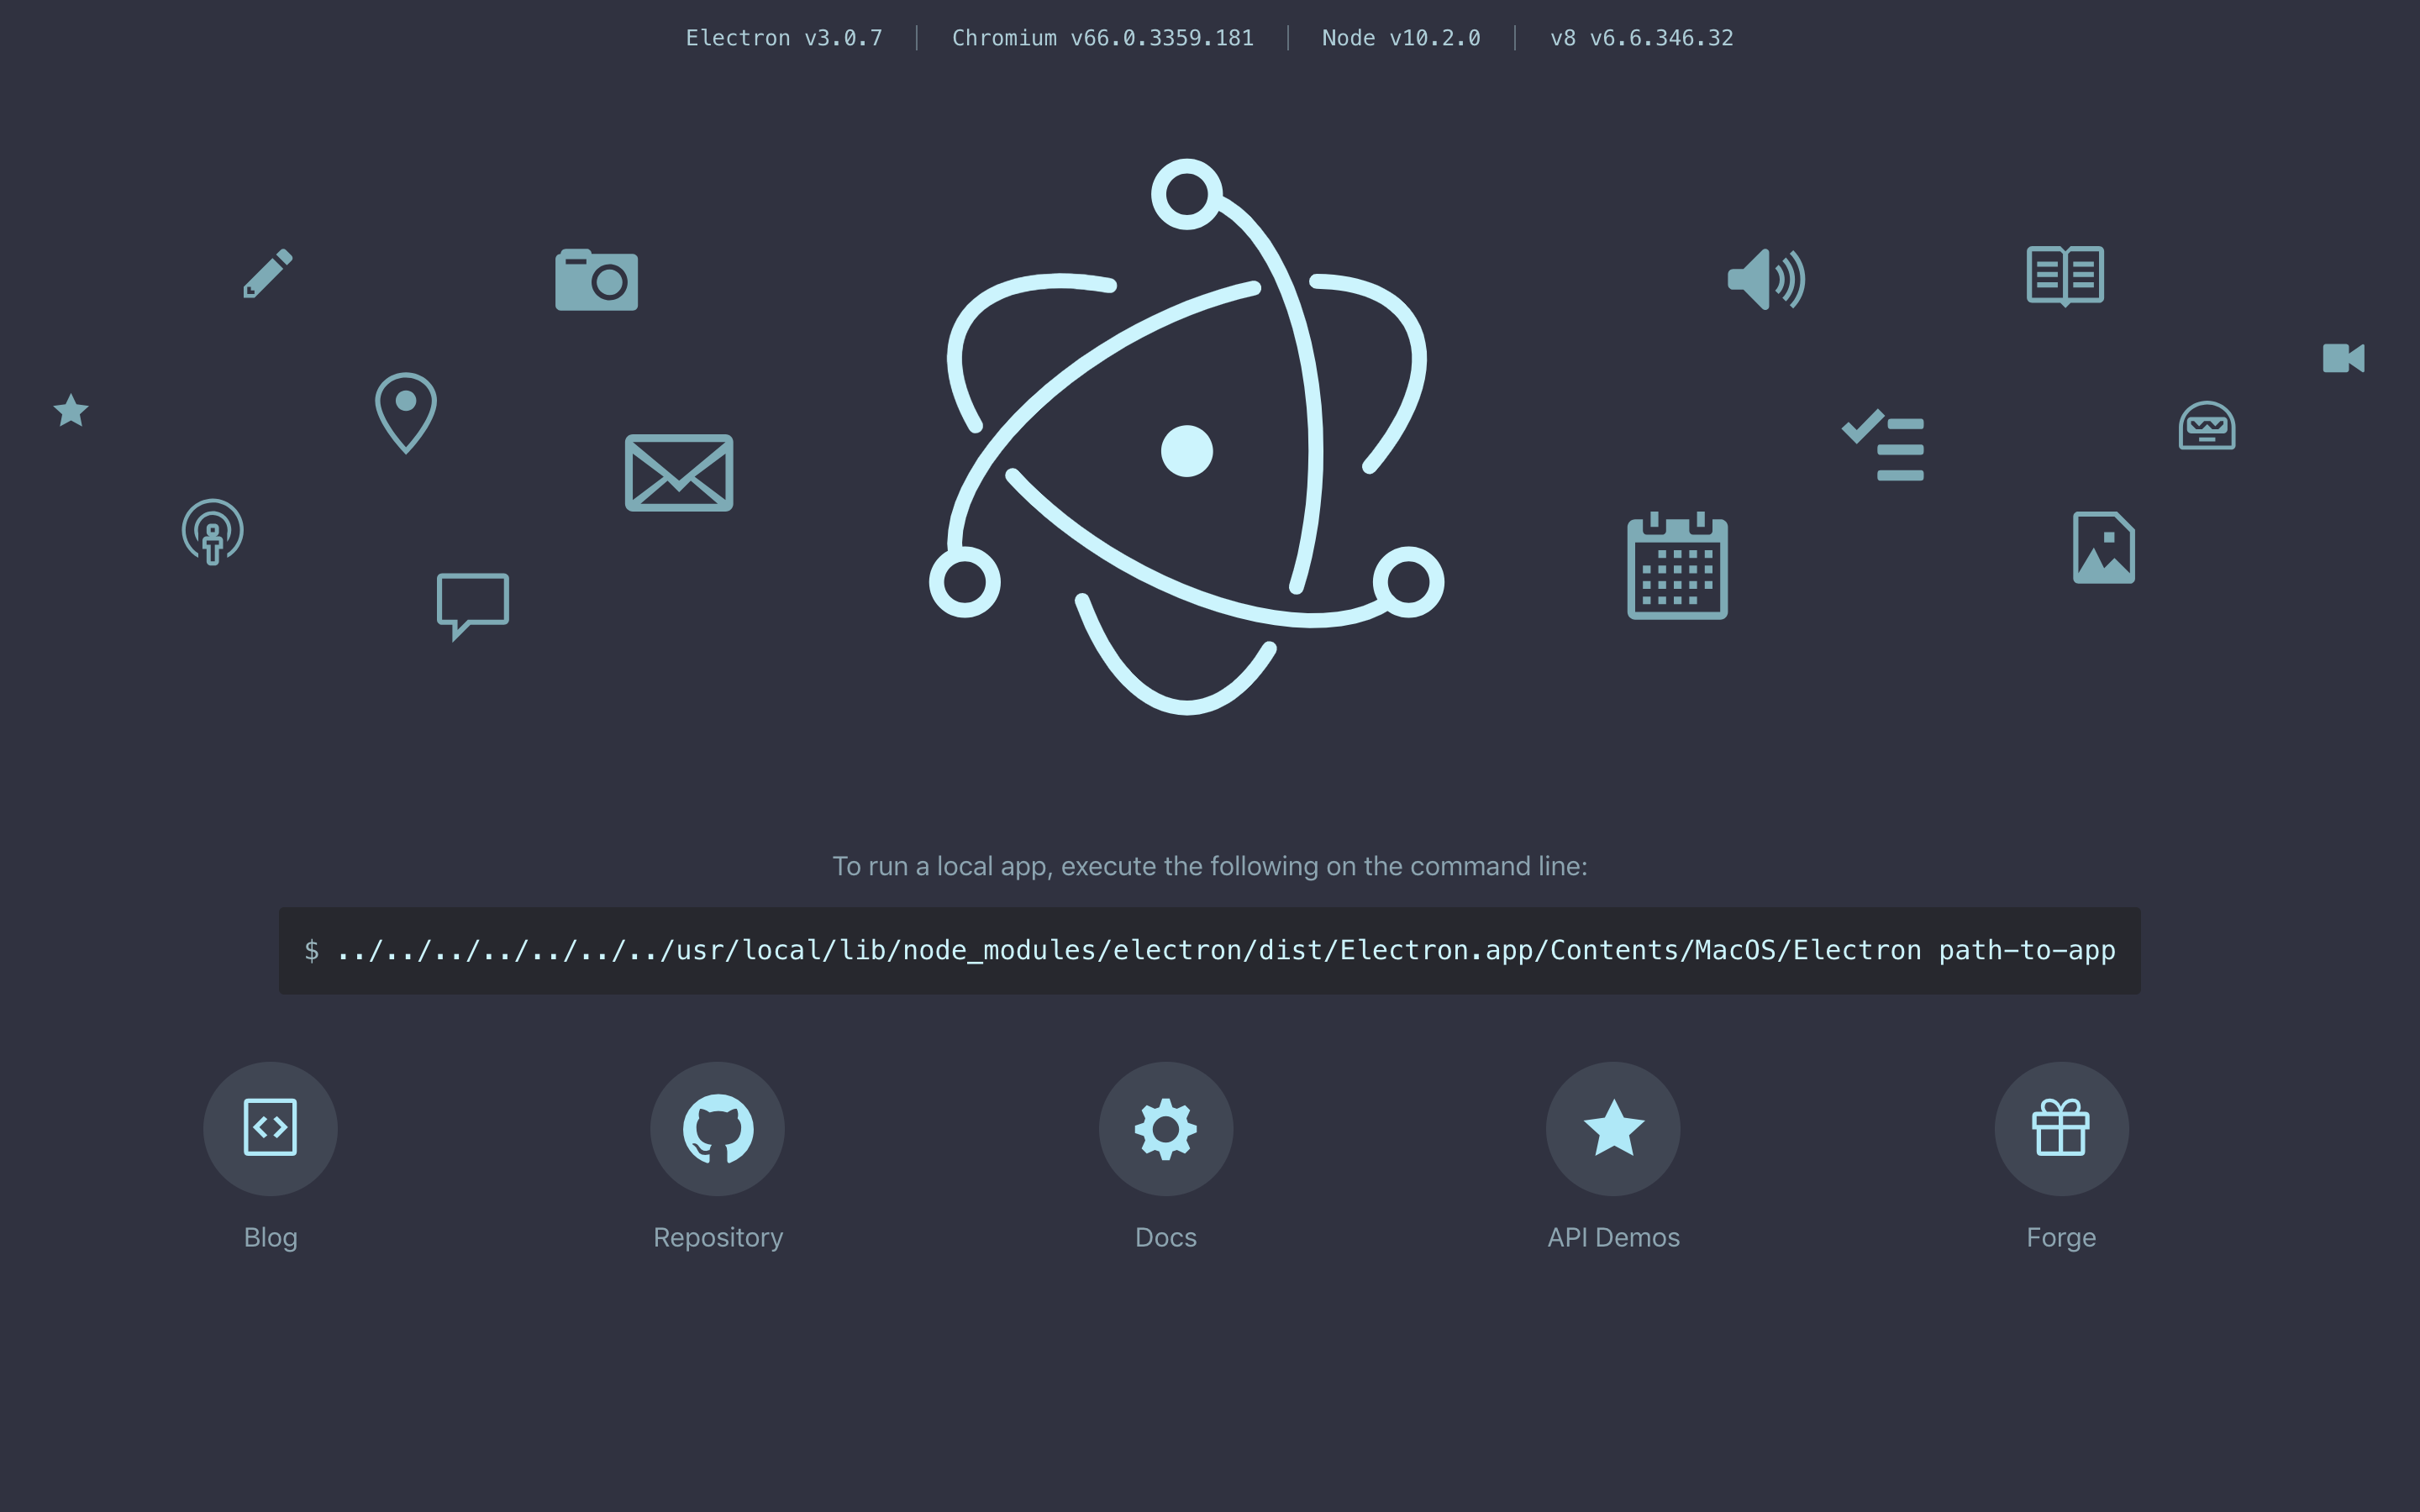
\includegraphics[width=\linewidth]{electron.png} % Figure image
	\caption{Electron} % Figure caption
	\label{elec} % Label for referencing with \ref{bear}
\end{figure}

\begin{lstlisting}
$bash: mkdir Electron1; cd Electron1; npm init
  1 {
  2   "name": "electron1",
  3   "version": "1.0.0",
  4   "description": "First App",
  5   "main": "index.js",
  6   "scripts": {
  7     "test": "echo \"Error: no test specified\" && exit 1"
  8   },
  9   "keywords": [
 10     "Electron"
 11   ],
 12   "author": "Boitumelo Phetla",
 13   "license": "ISC"
 14 }
\end{lstlisting}

At this point, you'll need to install electron itself. The recommended way of doing so is to install it as a development dependency in your app, which allows you to work on multiple apps with different Electron versions. To do so, run the following command from your app's directory:

\begin{lstlisting}
$bash: npm install --save-dev electron
$bash: tree -L 1
			.
			|____________node_modules
			|____________package-lock.json
			|____________package.json

1 directory, 2 files
\end{lstlisting}

All APIs and features found in Electron are accessible through the electron module, which can be required like any other Node.js module:

\begin{lstlisting}
const electron = require('electron')
\end{lstlisting}

To avoid any huddles, try this simple example.

\begin{lstlisting}
# Clone the repository
$ git clone https://github.com/electron/electron-quick-start
# Go into the repository
$ cd electron-quick-start
# Install dependencies
$ npm install
# Run the app
$ npm start
\end{lstlisting}

\subsection{\href{https://www.meteor.com/install}{Meteor}}


\begin{figure}[h!]
	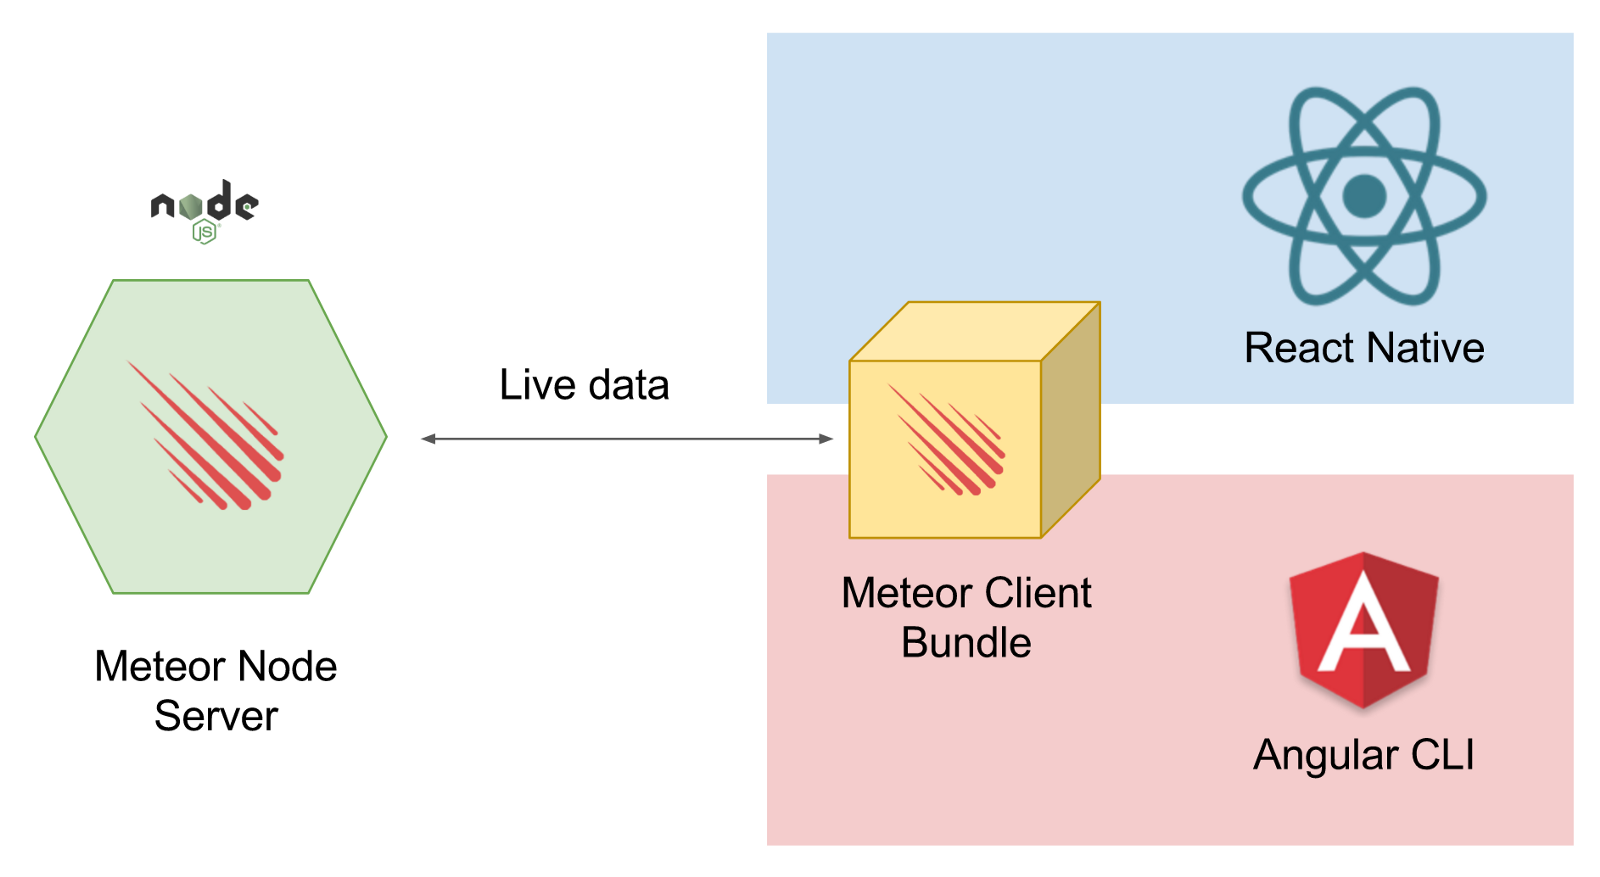
\includegraphics[width=\linewidth]{meteor.png} % Figure image
	\caption{Meteor} % Figure caption
	\label{mtr} % Label for referencing with \ref{bear}
\end{figure}

To create the app, open your terminal and type:

\begin{lstlisting}
$bash: meteor create simple-todos

output:

Created a new Meteor app in 'simple-todos'.                                        

To run your new app:                          
  cd simple-todos                             
  meteor                                      
                                              
If you are new to Meteor, try some of the learning resources here:
  https://www.meteor.com/tutorials            
                                              
To start with a different app template, try one of the following:

  meteor create --bare    # to create an empty app
  meteor create --minimal # to create an app with as few Meteor packages as possible
  meteor create --full    # to create a more complete scaffolded app

\end{lstlisting}


%------------------------------------------------

\subsection{JavaScript Editors (IDEs)}



\begin{itemize}
	\item \href{http://plnkr.co/edit/?p=catalogue}{Plunker}
	\item Second item in a list
	\item Third item in a list
\end{itemize}



%----------------------------------------------------------------------------------------
%	BIBLIOGRAPHY
%----------------------------------------------------------------------------------------

\printbibliography[title={Bibliography}] % Print the bibliography, section title in curly brackets

%----------------------------------------------------------------------------------------

\end{document}
